\documentclass{article}


\usepackage{arxiv}

\usepackage[utf8]{inputenc} % allow utf-8 input
\usepackage[T1]{fontenc}    % use 8-bit T1 fonts
\usepackage{hyperref}       % hyperlinks
\usepackage{url}            % simple URL typesetting
\usepackage{booktabs}       % professional-quality tables
\usepackage{amsfonts}       % blackboard math symbols
\usepackage{nicefrac}       % compact symbols for 1/2, etc.
\usepackage{microtype}      % microtypography
\usepackage{multirow}  % and items that fill up multiple rows in tables
\usepackage{graphicx}
\usepackage{xcolor,colortbl} % to add table color
\graphicspath{ {./images/} } % path to images
\usepackage{array} % add verticle space to tables
% to set up lists in tables to be left aligned:
\usepackage{enumitem}
\usepackage{tabularx}
\usepackage{etoolbox}
\usepackage{array}
\newcolumntype{P}[1]{>{\centering\arraybackslash}p{#1}}
\AtBeginEnvironment{table}{%
    \setlist[itemize]{nosep,     % <-- table's list setup
                      leftmargin = *         ,
                      label      = $\bullet$ ,
                      before     = \vspace{-0.6\baselineskip},
                      after      = \vspace{-\baselineskip}
                        }
                           }% end of AtBeginEnvironment
                           
\renewcommand{\arraystretch}{1.1} %adding space between rows will influence the rest of the document

\title{Impact of software designed for biomedical research: Are we measuring what's important?}




\author{
Spyridon Bakas \\
    University of Pennsylvania \\
    Philadelphia, PA 19104 \\
    \texttt{sbakas@upenn.edu} \\
\AND
David Hanauer \\
    University of Michigan Medical School\\
    University of Michigan School of Information\\
    Ann Arbor, MI 48109\\
    \texttt{hanauer@umich.edu}
\AND
Carrie Wright \\
    Fred Hutchinson Cancer Center
    Seattle, WA 98109 \\
    \texttt{cwright2@fredhutch.org}\\
}


  %% \AND
  %% Coauthor \\
  %% Affiliation \\
  %% Address \\
  %% \texttt{email} \\
  %% \And
  %% Coauthor \\
  %% Affiliation \\
  %% Address \\
  %% \texttt{email} \\



\begin{document}

 STILL WORKING OUT THE ORDER OF AUTHORS
 

\maketitle
Author list (currently alphabetically still figuring out what it will be - but will try to be based on amount of contribution):
Spyriodon Bakas, Paul Boutros, Greg Caporaso,  Guilherme Del Foil, James Eddy, Andrey Fedorov, Alex Getka, Mary Goldman, Brian Haas, David Hanauer, Harry Hochheiser, Aaron Holmes, Andrey Ivanov, Dan Knight, Martin Morgan, Sarthak Pati, Michael Reich, Pat Schloss, Levi Waldron, Jake Albrecht, (and members of ITN team)

% Use letters for affiliations, numbers to show equal authorship (if applicable) and to indicate the corresponding author



%\author[4, \Letter]{A. Afiaz}
%\author[4, \Letter]{Andrey Ivanov}
%\author[1,\Letter]{Savonen, C. L.}
%\author[2,\Letter]{Hanauer, D.}
%\author[3,\Letter]{Spyridon, B.}
%\author[4, \Letter]{Harry Hochheiser}
%\author[4, \Letter]{Greg Caporaso}
%\author[4, \Letter]{Guilherme Del Fiol}
%\author[4, \Letter]{James Eddy}
%\author[4, \Letter]{Paul Boutros}
%\author[4, \Letter]{Alex Getka}
%\author[4, \Letter]{Mary Goldman}
%\author[4, \Letter]{Martin Morgan}
%\author[4, \Letter]{Michael Reich}
%\author[4, \Letter]{Brian Haas}
%\author[4, \Letter]{Aaron Holmes}
%\author[4, \Letter]{Dan Knight}
%\author[4, \Letter]{Sarthak Pati}
%\author[4, \Letter]{Andrey Fedorov}
%\author[4, \Letter]{Pat Schloss}
%\author[4, \Letter]{Levi Waldron}
%\author[4, \Letter]{Jake Albrecht}
%\author[1,\Letter]{Leek, J. T.}
%\author[1,\Letter]{Wright, C.}
%\affil[1]{Fred Hutchinson Cancer Center}
%\affil[2]{University of Michigan Medical School\\ University of Michigan School of Information\\}
%\affil[3]{University of Pennsylvania}
%\affil[4]{Placeholder}

\begin{abstract}
Software has become vital for the advancement of biology and medicine. Analysis of usage and impact metrics of such software can help determine user and community engagement. These can be used to justify additional funding, encourage additional use, and identify unanticipated use cases. Such analyses can help define improvement areas and assist with managing project resources. However, there are challenges associated with assessing usage and impact, many of which vary widely depending on the type of software being evaluated. These challenges involve issues of distorted, exaggerated, understated, or misleading metrics, as well as ethical and security concerns.  More attention to the nuances, challenges, and considerations involved in capturing impact across the diverse spectrum of biological software is needed. Although some principles are generally applicable, there is not a single perfect metric or approach to effectively evaluate a software tool’s impact, as this depends on aspects unique to each tool, how it is used, and how one wishes to evaluate engagement. We propose generalizable guidelines, as well as strategies for various types of software and resources. We also highlight outstanding issues in the field regarding how communities measure or evaluate software impact. To gain a deeper understanding of the issues hindering software evaluations, as well as to determine what appears to be helpful, we performed a survey of participants involved with scientific software projects for the Informatics Technology for Cancer Research (ITCR) program funded by the National Cancer Institute (NCI). We also performed investigations of software among this scientific community and others to determine how often infrastructure that supports such evaluations is implemented and how this impacts citation rates. We  find that although developers recognize the utlility of analyzing the usage of their software, they struggle to find the time or funding to support such analyses. We also find that infrastructure such as social media presence, more in-depth documentation, the presence of software health metrics, and clear information on how to contact developers seem to be associated with increased citation rates.  Our findings can help scientific software developers make the most out of the evaluations of their software so that they can more fully benefit from such assessments.
\end{abstract}


% keywords can be removed
%\keywords{First keyword \and Second keyword \and More}


\section{Introduction} Biomedical software has become a critical component of nearly all biomedical research. The field has embraced more open science practices, including sharing and harmonizing data and creating open source (publicly accessible and often freely available) software \cite{green_strategic_2020, levet_developing_2021, itcr_open-source_2021, merow_better_2023}. Often such open source software is initially developed so that the developers can use it themselves to reach a research goal \cite{bitzer_intrinsic_2007}. The software is then shared with the hopes that the use of the software by others will also contribute to the advancement of science or healthcare. Once shared, evaluations of the software is necessary to achieve two major benefits: 1) inform developers about how to improve the use and ultimately impact of the tool and 2) demonstrate the value of the tool to support the developers to obtain funding to continue supporting existing software and creating new software. Common metrics include number of new users, returning users, and total downloads of the software, but the type of metrics possible vary based on the type of tool and the context. See Table ~\ref{tab:metrics_table}. These and other metrics, allow assessment of the rate of uptake of a tool, as well as how established it has become. However, developers often lack knowledge about the infrastructure or tools that can aid in the effective collection of usage and impact metrics. Proper metrics should not only examine the software's performance but assess whether motivations and goals of the researchers who are using the software are being met.

\begin{table}[h!]
 \caption{Common Metrics}
  \centering
  \begin{tabular}{|p{0.2\textwidth}|p{0.25\textwidth}|p{0.3\textwidth}|}
    \hline
    \multicolumn{1}{|c|} {\cellcolor[gray]{.9} \textbf{Measure}} 
    & \multicolumn{1}{|c|} {\cellcolor[gray]{.9} \textbf{Example Metrics}}     
    & \multicolumn{1}{|c|} {\cellcolor[gray]{.9} \textbf{Use}}  \\
    \hline
    \multirow{4}{*}{Tool Dissemination} 
    & 
     \begin{itemize}
         \item Total unique downloads
         \item New Users
         \item Returning Users
         \item Download count by version
     \end{itemize} &
    \begin{itemize}
         \item Determining popularity of a given tool
    \end{itemize}  \\ 
           \cline{2-3}
    &     
    \begin{itemize}
         \item Download count by version
    \end{itemize}  &
    \begin{itemize}
         \item Assessing if users are keeping up-to-date
 \end{itemize}  \\ 

    \hline
    Tool Usefulness & 
    \begin{itemize}
         \item Average run count, by user
    \end{itemize}  &
    \begin{itemize}
         \item Determining prevalence of usage
    \end{itemize} \\
    \hline
    Tool Reliability & 
    \begin{itemize}
         \item Proportion of runs without a crash or error
    \end{itemize}  &
    \begin{itemize}
        \item Improving error handling, bug fixes 
    \end{itemize} \\
    \hline
    Tool Versatility &
        \begin{itemize}
        \item Distribution of data types (inferred from metadata) 
        \end{itemize} &
        \begin{itemize}
        \item Improving tool flexibility
        \end{itemize}\\
    \hline
    Interface acceptability &
    \begin{itemize}
        \item Average user session length
    \end{itemize} &
    \begin{itemize}
        \item Graphical tool and website acceptability
        \end{itemize}\\
    \hline
    Performance &
    \begin{itemize}
        \item Maximum memory usage
        \item Average time-to-complete of algorithmic steps 
    \end{itemize} &
    \begin{itemize}
        \item{Requirements analysis}
        \item{Tuning}
    \end{itemize}\\
    \hline
  \end{tabular}
  \label{tab:metrics_table}
\end{table}

We aim to provide guidance for evaluations of software impact and engagement so that software developers can build tools that better meet researchers' needs to catalyze the progress of biomedical research. We also discuss ethical considerations and challenges of such evaluations that still require solutions. The guidance presented here for software assessments holds the potential for developers to improve the use and utility of their tools, improve their chances of funding for future development, and ultimately lead to the development of even more useful software to advance science and medicine \cite{wratten_reproducible_2021}. 



\section{Assessment of attitudes and practices for software impact evaluations}

We performed two analyses to better understand how developers think about software evaluation and to determine what infrastructure is often implemented to support such evaluation, as well as how this is associated with citation levels among those of the Informatics Technology for Cancer Research (ITCR) program funded by the National Cancer Institute (NCI). 

To perform the first analysis we surveyed 48 ITCR participants. The survey asked a variety of questions about attitudes and practices of those involved with software development, maintenance, or outreach of the ITCR (in which respondents could often select more than one response). It was determined that limited time (68.1\% of respondents) and funding (57.4\% respondents) were the major barriers for performing software impact evaluations. Indeed although there are a few funding mechanisms that support the maintenance and analysis of software (as opposed to creation of new software), such as the Informatics Technology for Cancer Research (ITCR) program funded by the National Cancer Institute (NCI) sustainment awards \cite{kibbe_cancer_2017, warner_informatics_2020} or the Essential Open Source Software for Science program of the Chan Zuckerberg Initiative \cite{CZ_essential_2019}, there appears to be a need for greater support. The next major barriers were privacy concerns (38.3\% of respondents), technical issues (31.9\% of respondents), and not knowing what methods to use for such evaluations (27.2\% of respondents). Despite these apparent challenges,  72.9\% of respondents state that such evaluations have informed new development ideas, 60.4\% stated that it informed documentation, and 54.2\% stated that it helped justify funding.  Thus additional support, could really benefit the continued development of software. Aspects that respondents had difficulty measuring were:
\begin{itemize}
    \item Collaborations that the tool supported
    \item Number of commercial applications using the tool
    \item Fraction of assumed user base that actually uses the tool
    \item Downstream activity - what do users do with the results
    \item User Frustration
\end{itemize}

We also manually inspected 44 tools (33 funded by ITCR alone and 7 funded by the Cancer Target Discovery and Development (CTD²) Network \cite{aksoy_ctd2_2017}, as well as 4 tools funded by both) for various aspects and investigated if there were any associations with these aspects and funding. A variety of tools were inspected - See Figure \ref{fig:tool_eval}. Most notable was a finding that although time since tool release is the largest contributor to variation of citations that report actual usage, various aspects of infrastructure that could help users know about a tool (social media on twitter), have confidence in the tool (badges about software builds or tests on code repositories), or learn more about how to use the tool (extensive documentation and feedback mechanisms), all seem to increase the rate of manuscripts that describe using the tool and officially cite the tool.See Figure \ref{fig:inf_cit}

\begin{figure}[!ht] 
    \centering
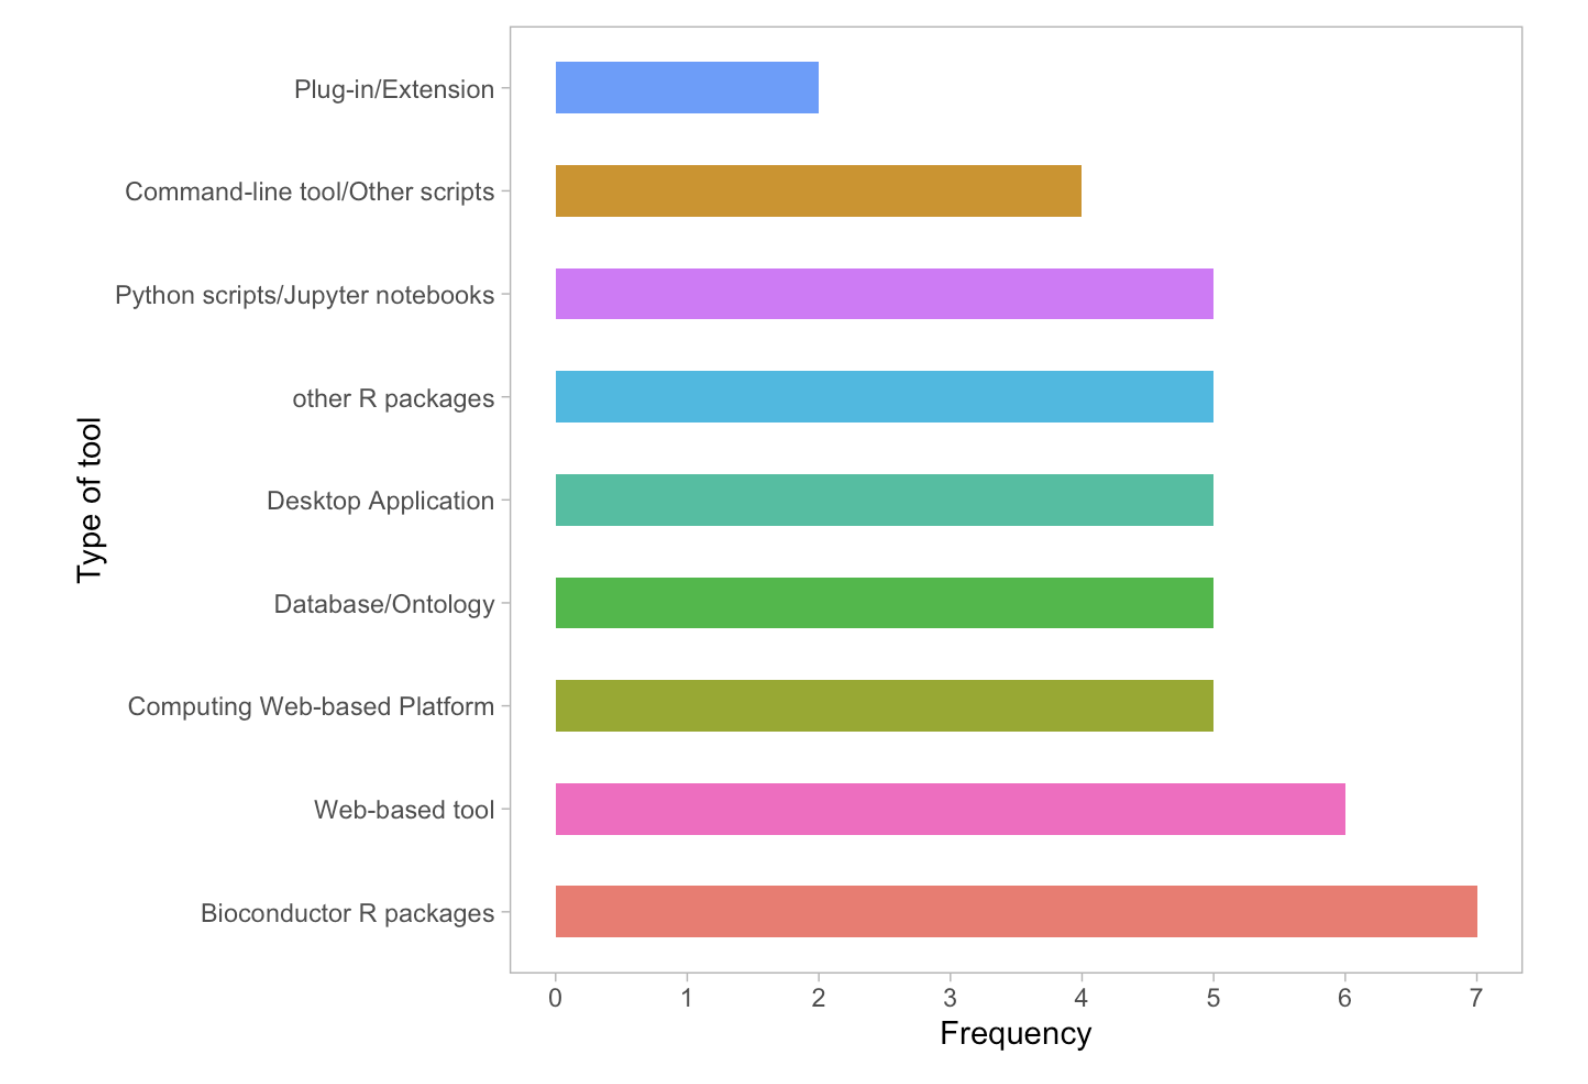
\includegraphics[width=\textwidth,height=\textheight,keepaspectratio]{images/tool_diversity.png}
    \caption{Variety of the 44 ITCR and CTD² tools evaluated for various characteristics with manual inspection}
    \label{fig:tool_eval}
\end{figure}



\begin{figure}[!ht]
    \centering
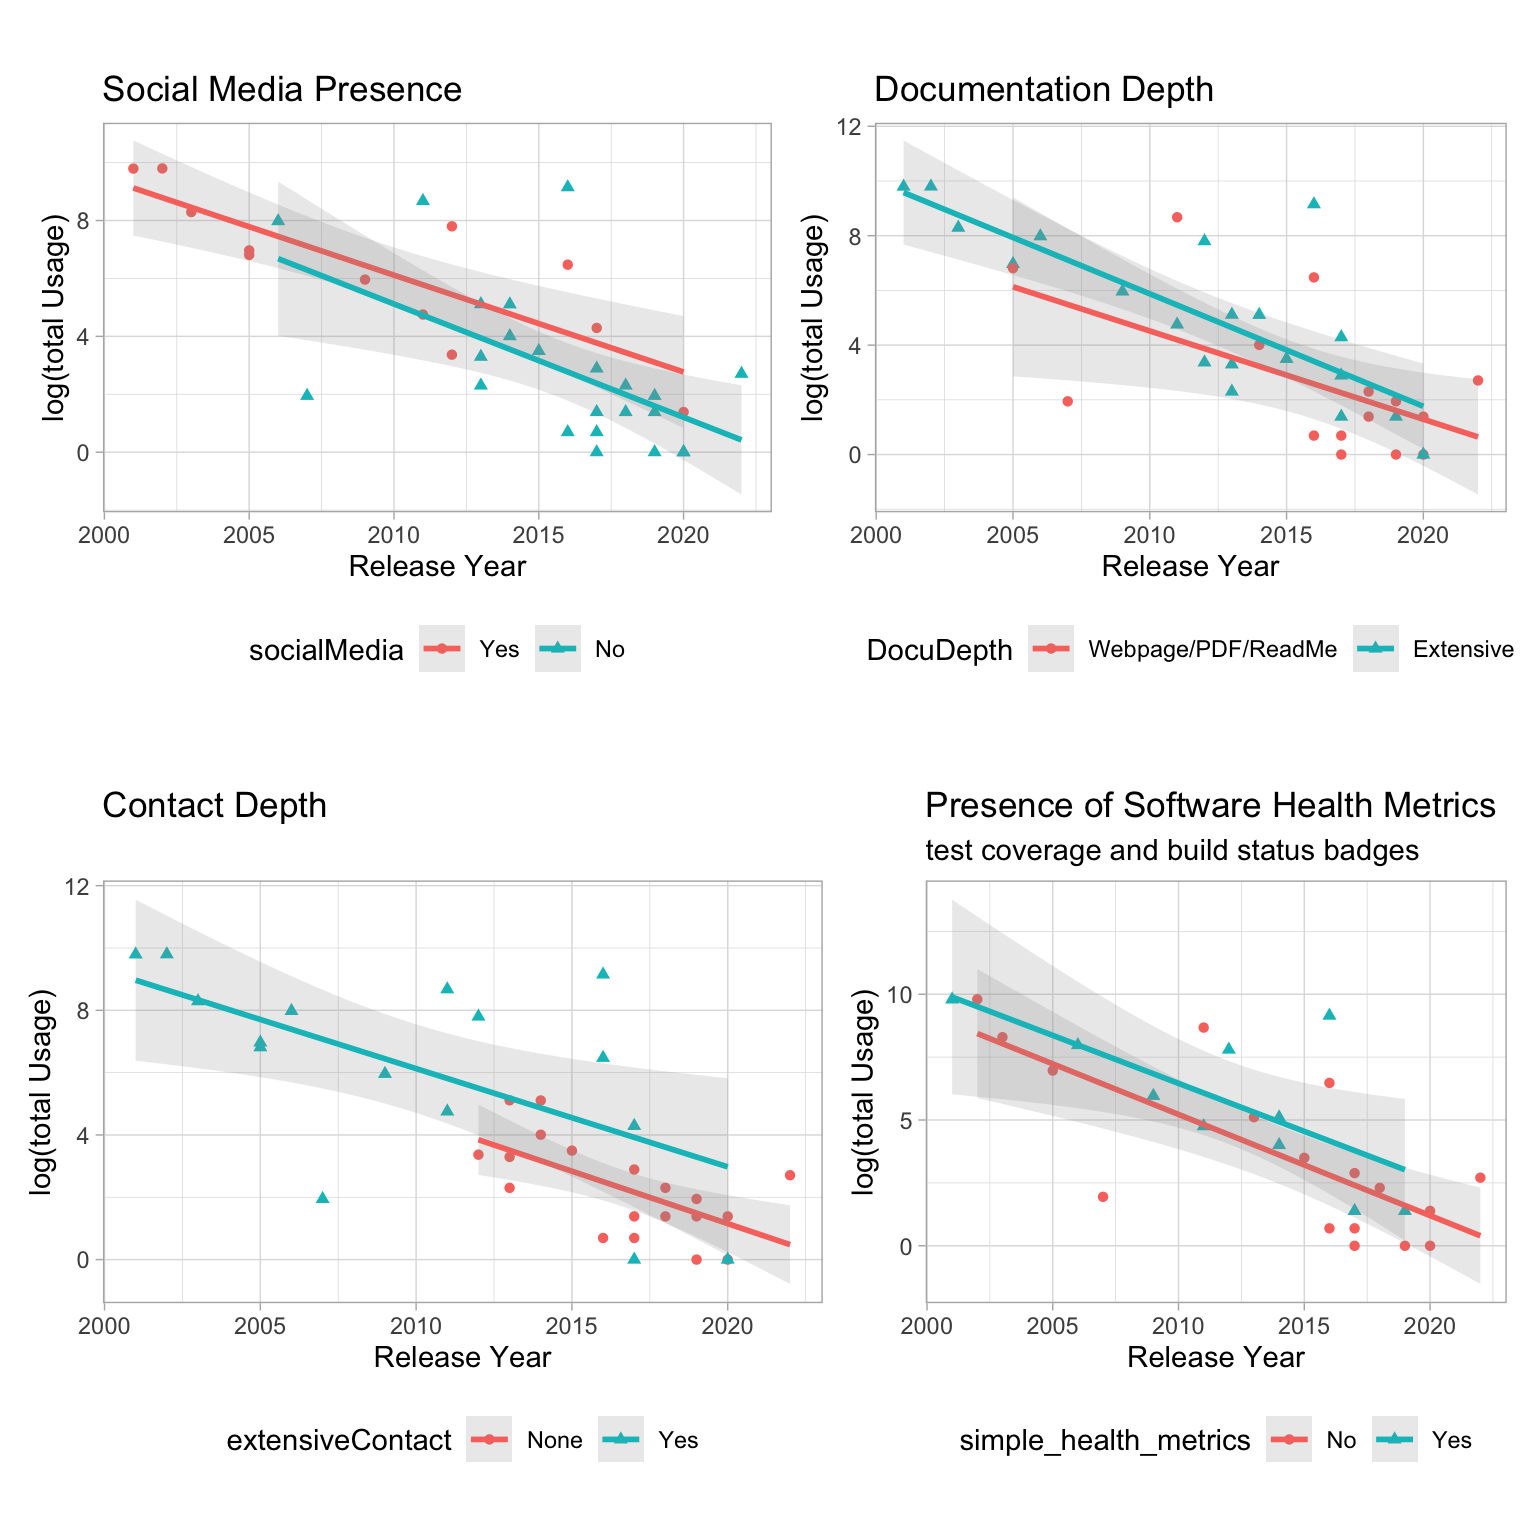
\includegraphics[width=\textwidth,height=\textheight,keepaspectratio]{images/inf_cit.png}
    \caption{Various aspects of software infrastructure appear to be associated with a larger number of published manuscripts from users officially citing usage of the software.}
    \label{fig:inf_cit}
\end{figure}



\section{Overall guidance}





\subsection{Successful evaluations are anchored by an understanding of the intended use of the software}
\label{sec:use_understanding}
The intended goal or purpose of the scientific software should be used to inform how the software is evaluated. Computational tools are designed to support well-defined goals often called use cases \cite{gamma_design_1995} for specific sets of users called personas\cite{cooper_inmates_2004}. Efforts to evaluate the impact of tools should be guided by a clear understanding of these use cases and personas to assess how well the tools meet the intended goals.  

\subsection{Metric selection should be hypothesis driven} 
\label{sec:hypothesis_driven}
Collecting an exhaustive amount of user data, and then selecting metrics, can add complexity and increase the risk that metrics are selected in a biased manner. To mitigate this, metrics can be selected ahead of time based on a specific hypothesis to ultimately evaluate how well the software supports it’s intended goals. 


\subsection{Intentions for evaluation can also inform design choice} Software can also be designed with future evaluations in mind. Once the intended use of the software is clearly defined, avenues for what to investigate in terms of usage will also become clear. For example, Xena \cite{xena_2020} is a tool intended to enable users to visualize various aspects of the genome. The developers collect metrics involving how often users use the tool to perform  visualizations. However consideration of privacy led the developers to not collect metrics about what part of the genome gets visualized. 




\subsection{Metrics can achieve different goals for different audiences}

Clear understanding of which use cases, personas, and audience(s) are of interest, as well as what motivations are of interest, can help guide what user metrics to collect to achieve project goals.  For example, if the audience is the developers themselves, and the motivation is to learn how to retain new users, it may be helpful to understand how well new users are able to learn the basics of the tool. Thus focusing on metrics related to interactions with tutorials may be the most useful. These measurements might be very different from metrics used to understand which scripting features are being used by advanced users. 

It is also worthwhile to consider which presentations of software metrics will be most compelling to the intended audience. For example, detailed metrics on the inner workings of a software tool might be highly-informative to developers, but such metrics would be far too granular to be of interest to funding agencies.  See \ref{tab:benefit_table} for more details.
 
\begin{table}[ht!]
 \caption{\textbf{Software evaluation supports internal needs for tool optimization and development, as well external needs to demonstrate tool value 
 to others.} Tool optimization can involve improving workflows, performance, usage, or usability. Evaluations can guide future work. For example, recognizing the types or volumes of data being used, as well as temporal trends of data usage, can highlight opportunities for new algorithm development. Similar analyses can help optimize resource allocation within and between projects. Evaluation can also aid in demonstrate tool value to gain external support, such as funding.  Evidence for impact is also often required to gain resources to develop or maintain semi- or un-related tools. Demonstration of past capability to develop impactful software supports requests to do so in the future.  Demonstrating that a tool is widely-used and widely-accepted can also encourage users to adopt a tool more readily, and be more invested in a tool community. Developers may be drawn to projects with impact to build upon an exiting tool. Finally, demonstration of impact can recruit new users which can diversify tool communities and bring new problems of interest that expand the utility of a tool.}
  \centering
  \begin{tabular} {|p{0.27\textwidth}|p{0.25\textwidth}|p{0.4\textwidth}|}
  %{|c|c|l|}
    \hline
    \multicolumn{1}{|c|}{\cellcolor[gray]{.9} \textbf{Internal Need}} 
    & \multicolumn{1}{|c|}{\cellcolor[gray]{.9} \textbf{Specific Goal}}
    & \multicolumn{1}{|c|}{\cellcolor[gray]{.9} \textbf{Benefit}}\\[1.1ex]
    \hline
    \multirow{17}{*}{Tool Optimization}               
    & \multirow{3}{*}{Improving Workflows} & 
    Identify unexpected usage \\
    & &
    Identify code inefficiencies \\
    & &
    Identify resource usage inefficiencies \\
    &&
    Identify inadequate documentation\\ \cline{2-3}
    &   \multirow{4}{*}{  }
    & 
     Identify mismatches with defaults and use \\
     &  Improve Performance  &
    Assess user wait times \\
    &  & 
     Measure data volume \\  \cline{2-3}
    & \multirow{5}{*}{ Improve Usage} & 
    Identify software errors \\
    &&
    Identify what features are used and not used \\
    &&
    Identify who the user-base is \\
    & &
    Determine user-base diversity \\
    & &
    Identify sources of other possible users \\
    & &
    Determine what users expectations are \\
    & &
    Determine if user expectations are appropriate \\
    & &
    Evaluate success of outreach approaches\\  \cline{2-3}
    & \multirow{2}{*}{ Improve Implementation} & 
    Identify barriers for adoption \\
    &   &
    Identify methods to support adaption \\
    &  & 
    Identify use of out-dated versions\\\cline{2-3}
    & \multirow{2}{*}{ Improve Usability} & 
    Identify user errors \\
    & & 
    Identify if and how users are struggling \\ 
    \hline
    \multirow{6}{*}{\shortstack{Tool Development \\ \& Maintenance}}
    & \multirow{6}{*}{\shortstack{ Guide Future Work\\  Motivate Continued Support}} &
    Enumerate data types being used \\
    & &
    Discover opportunities for new features \\
    && 
    Discover data needed to address user goals  \\
    & & 
    Identify more appropriate resource allocation \\

    \hline
    \multicolumn{1}{|c|}{\cellcolor[gray]{.9} \textbf{External Need}} 
    & \multicolumn{1}{|c|}{\cellcolor[gray]{.9} \textbf{Specific Goal}}
    & \multicolumn{1}{|c|}{\cellcolor[gray]{.9} \textbf{Benefit}}\\[1.1ex] % add some space after headers before horizontal line
    \hline
    \multirow{4}{*}{Gain Support}              
    & \multirow{4}{*}{Show Evidence of Impact} & 
    Support future funding requests \\
    & &
    (to maintain or develop new tools) \\
    & &
    Request for resources  \\
    & & 
    (to maintain or develop new tools) \\[1.1ex]
    \hline
    \multirow{4}{*}{Gain User Commitment} 
    & \multirow{4}{*}{Evidence of tool acceptance} & 
    Reassure users about tool to:\\
    &&
    - Promote continued use\\
    && 
    - Promote usage of new tools by the same developers \\ 
    &&
    - Promote usage by more diverse users \\[1.1ex]
    \hline
    \multirow{1}{*}{Gain Community Development} 
    & \multirow{1}{*}{Evidence of co-development} & 
    Encourage contributions  \\
    \hline
  \end{tabular}
  \label{tab:benefit_table}
\end{table}

\subsection{No single evaluation method works for every type of software}
\label{sec:no_one_way}
No individual scheme for collecting metrics fits every type of research software tool.  The meaning of a set of metrics may differ across contexts. The location of a tool (e.g., whether it is on the web or downloaded) can affect metric collection and influence user access to software versions. For example, for a web-based application, it may be feasible to collect user metrics on a per-account basis and to collect information about the type of data or software features users tend to work with. With web-based tools, users will rarely have access to older versions of the software. Thus developers can add version updates and collect metrics with clarity about how usage changed with updates. On the other hand, for tools that must be run (and possibly installed)  locally, users may be using older versions of the software that they previously downloaded.  Here, metrics on a per-version basis provide a much better representation of usage, rather than simply the overall number of unique downloads. Collection of version usage is important, as developers may want to pair this with citation data to know if users are using out-of-date aspects of previous versions of the software.



 \subsection{Metrics should be interpreted}
 
 Interpretation of user metrics can be tricky since any given metric may have many obvious and not so obvious causes. When software has sufficient use, observed spikes in usage, both up and down, provide important feedback. A spike may correspond to a class or workshop using the tool or a recent publication that cites the tool. Negative trends in usage may indicate a break in the academic calendar, down time of a host server, or, for tools based on Amazon Web Services, the additional compute resources required by Amazon during holiday cycles may preempt software running on spot instances. It is also important to avoid comparisons between metrics for tools with different users. For example, clinical tools that require institutional will have lower installation rates than other software tools. Tools that are very useful to a small number of users may still have important impact on the field.

The total unique downloads might be useful as a metric of software popularity, but it only reflects how many people have tried to download it and not if users find it useful. Instead, one might consider measuring how often users use software, we might count the number of launches of the software which run over a certain predefined session time threshold,to better evaluate actual usage. Returned usage by the same users often suggests that the users may find the tool useful. One may want to parse this by data type used to evaluate how useful the tool appears to support different kinds of users.   Specific measures can provide common basis comparing versions and potentially against other similar software.


\subsection{Software infrastructure enables impact evaluation}
There are several components of a software tool that can assist with the assessments of the software impact and engagement. Once a developer team better understands their audience, use cases, personas, and assessment motivations, the following infrastructure could benefit or enable such evaluations, as well as improve user awareness and engagement. 
See Table~\ref{tab:inf_table} and supplementary note 1 for suggestions.

\begin{table}[ht!]
 \caption{\textbf{Software infrastructure enables the capture of valuable metrics for evaluating engagement and impact.} Note that there are other helpful tools to enable metric collection. Those listed are simply examples. }
  \centering
  \begin{tabular} {|p{0.03\textwidth}|p{0.18\textwidth}|p{0.18\textwidth}|p{0.23\textwidth}|p{0.24\textwidth}|}
    \hline
    \multicolumn{1}{|c|}{\cellcolor[gray]{.9} \textbf{Elements}} 
    & \multicolumn{1}{|c|}{\cellcolor[gray]{.9} \textbf{Options}}
    & \multicolumn{1}{|c|}{\cellcolor[gray]{.9} \textbf{\shortstack{\\Tools to Enable \\Metric Collection}}}
    & \multicolumn{1}{|c|}{\cellcolor[gray]{.9} \textbf{\shortstack{\\Possible\\ Enabled Metrics}}}
    & \multicolumn{1}{|c|}{\cellcolor[gray]{.9} \textbf{Considerations}}\\[1.1ex]
    \hline
    \multirow{8}{*}{\shortstack{Web \\ Presence}}               
    &   \multirow{2}{*}[-2em]{ Web-based tool} & 
    \raggedright{
    \begin{itemize}
        \item Cronitor \cite{cronitor} for tools using cron job scheduling \cite{cron_2009})
        \item Google Analytics\cite{google_analytics}
    \end{itemize}
    }
    & 
    \begin{itemize}
    \item Identify details about usage
    \item Identify where your tool is being used
    \item Possibly identify what data is being used
    \end{itemize} &  May need to consider privacy restrictions for tracking IP addresses\\
    \cline{2-5}
    & \multirow{2}{*}[-1em]{ \shortstack{Documentation \\ Website}} &
    \begin{itemize}
        \item Google Analytics\cite{google_analytics}
    \end{itemize}
    &
    \begin{itemize}
    \item Counts of page views and scrolls
    \end{itemize} &
    Pages with more views may identify widely used features or confusing aspects \\
    \hline
    \multirow{3}{*}[-2em]{Citability}
    & \raggedright{Providing something to cite (Software DOI or manuscript) and information on how to cite} & \raggedright{
    \begin{itemize}
        \item To create DOIs: Zenodo \cite{zenodo}, Dryad \cite{datadryad}, Synapse \cite{synapse}, and Figshare \cite{figshare} 
        \item To track DOIs: Altmetric \cite{noauthor_altmetric_2015}
    \end{itemize}} &
     \begin{itemize}
         \item total citation counts 
         \item counts of citations in by journals of different fields
     \end{itemize} & Semantic Scholar \cite{noauthor_semantic_nodate} provides reports that indicate where citations have occurred within scientific articles. \\
        \hline
    \multirow{3}{*}[-5em]{Contact} &
    \multirow{3}{*}{\shortstack{\\Feedback \\Mechanisms}} & 
    \begin{itemize}
    \item GitHub Issue Templates
    \item Surveys
    \end{itemize}
    & 
    \begin{itemize}
    \item User feedback count
    \item addressed user feedback count 
    \end{itemize} & Often users will only provide feedback if something is broken. Depending on the tool, many users may not be comfortable with GitHub Issues\\
    \cline{2-5}
    & \multirow{2}{*}{ \shortstack{Discussion \\ Forums}} &
    \begin{itemize}
        \item Discourse \cite{discourse}
        \item Biostar \cite{biostars}
        \item Bioinformatics Stack Exchange \cite{bioinformaticsstackexchange}
    \end{itemize} &
    Metrics based on user engagements and answered questions & Forums save time for development as users help each other instead of developers answering individual emails for repeat problems. A code of conduct can help create a supportive community.\\
    \cline{2-5}
    & \multirow{2}{*}{ \shortstack{Newsletter\\Emails}} &
    \begin{itemize}
        \item Mailchimp \cite{mailchimp}
        \item HubSpot \cite{hubspot} 
    \end{itemize} & 
    \begin{itemize}
        \item count of newsletter openings
        \item count of link clicks
        \item count of unsubscribers
    \end{itemize} & Newsletters can help inform users about new features \\
    \hline
    \multirow{3}{*}{\shortstack{Usability\\Testing}}
    & \raggedright{Observe a few people use the tool} & 
    \begin{itemize}
        \item Zoom screen sharing and recording
    \end{itemize} & Qualitative information about how users interact with your software& Even low numbers of usability interviews (~3) can yield fruitful lessons that can be paired with other metrics to guide development\\
    \hline
    \multirow{3}{*}{Workshops}
    & \raggedright{ Online or in-person, Basics for new users or new features for existing users} & Attendees can participate in surveys &  Quantity, duration, and attendance at workshops are metrics that can be reported to funding agencies & Recordings of instructors can  be posted on Social Media (for additional metrics)\\
    \hline
    \multirow{3}{*}{\shortstack{Social\\ Media}}
    & \begin{itemize}
        \item YouTube Videos
        \item Twitter/mastodon
        \item Instagram
        \item LinkedIn 
    \end{itemize} & 
    \begin{itemize}
        \item Hootsuite \cite{hootsuite} - social media management
    \end{itemize} &   Engagement metrics (video watch counts, likes, etc)  & Pairing Social media  metrics with software engagement metrics can determine if outreach strategies are successful \\
    \hline
       \multirow{3}{*}{Reviews}
    & Review Forum & 
    \begin{itemize}
        \item SourceForge
        \item GitHub
    \end{itemize} &  \begin{itemize}
        \item Stars
        \item number of reviews
    \end{itemize} & Positive reviews can reassure new users and funders\\ 
    \hline
  \end{tabular}
  \label{tab:inf_table}
\end{table}



\subsection{Software project health metrics can reassure users and funders}
Tracking adherence to standards of software engineering can be a useful way to assess software project health including the use of version control systems, high coverage of code with testing, and use of automated or continuous integration. None of these measures of project health are perfect (and they can be done poorly) but overall they can be collectively assessed as indicators of software health. Including badges for such indicators on code repositories and websites can give users and others confidence in your tools.  Additional detail on these topics, can be found in The Pragmatic Programmer\cite{thomas_pragmatic_2019}. See Table~\ref{tab:soft_health_table} and supplementary note 2 for suggestions.


\begin{table}[ht!]
 \caption{\textbf{Software health infrastructure enables collecting metrics that can reassure users and funders.}  }
  \centering
  \begin{tabular} {|p{0.1\textwidth}|p{0.13\textwidth}|p{0.15\textwidth}|p{0.23\textwidth}|p{0.24\textwidth}|}
    \hline
    \multicolumn{1}{|c|}{\cellcolor[gray]{.9} \textbf{Infrastructure}} 
    & \multicolumn{1}{|c|}{\cellcolor[gray]{.9} \textbf{Options}}
    & \multicolumn{1}{|c|}{\cellcolor[gray]{.9} \textbf{\shortstack{\\Tools to Enable \\Metric Collection}}}
    & \multicolumn{1}{|c|}{\cellcolor[gray]{.9} \textbf{\shortstack{\\Possible\\ Enabled Metrics}}}
    & \multicolumn{1}{|c|}{\cellcolor[gray]{.9} \textbf{Considerations}}\\[1.1ex]
    \hline
    \multirow{6}{*}{Version Control}               
    &   \multirow{3}{*}[-3em]{\shortstack{Without\\ automation}} & \raggedright{\begin{itemize}
        \item Git/GitHub \cite{GitHub} (The insight tab and API allow for systematic metric collection)
        \item Git/GitLab \cite{GitLab}
        \item BitBucket \cite{bitbucket}
    \end{itemize}}
    & 
    \begin{itemize}
    \item Commit  frequency (how often code is updated)
    \item Date of the most recent commit
    \item Number of active contributors
    \item Software versions updates
    \end{itemize} &
     Commit frequency allows assessment of how actively the software is being maintained. The number of contributors can indicate sustainability. One single contributor may pose a sustainability risk. Version information can enable users to determine if they are using the most up-to-date version. \\
    \cline{2-5}
    & \multirow{5}{*}[-3em]{ \shortstack{With\\ Automations}} & \raggedright{
    \begin{itemize}
        \item GitHub Actions \cite{github_actions}
    \end{itemize}
    }
    &
    \begin{itemize}
    \item  current build status (if the software built without errors) 
    \end{itemize} &
    Continuous Integration \& Continuous Deployment/Delivery are terms to describe every time code is modified, the full code product is automatically rebuilt or compiled. Continuous Deployment/Delivery describes the automatic release of this new code to users. Delivery in this case describes situations where the software requires more manual releases while deployment is seamless. GitHub Actions can also help with metric collection from the GitHub API. \\
    \hline
    \multirow{3}{*}[-2em]{Testing} 
    & \multirow{2}{*}[-3em]{ \shortstack{Automated \\ Testing}} & \raggedright{
    \begin{itemize}
        \item GitHub Actions \cite{github_actions}
    \end{itemize}
    } &
    \begin{itemize} 
    \item test code coverage (the fraction of lines of code in the project that are covered by tests)
    \end{itemize} & Unit tests check individual pieces of code; component and integration tests check that pieces of code behave correctly together; acceptance tests check the overall software behavior. Achieving in-depth test coverage requires careful software design. Test coverage does not evaluate the quality of the test cases or assertions.\\
    \hline
    \multirow{3}{*}[-2em]{Licensing}
    & \raggedright{A variety of licenses exist to allow or disallow reuse and to require attribution} & \raggedright{
    \begin{itemize}
        \item Creative Commons \cite{creative_commons}
    \end{itemize}
    } & Possible quantification of reuse of your software code & Clearly indicating if and how people can reuse your code will make them more comfortable to do so. Determining when this is done can be a challenge, but requiring attribution makes this more feasible\\
    \hline
  \end{tabular}
  \label{tab:soft_health_table}
\end{table}




\section{Challenges and nuances}

There are a number of challenges and nuances associated with evaluating metrics for software usage and impact. Here we outline some examples.

\subsection{Citation challenges}
Measuring the number of citations of your tool is especially useful as a metric to report to funding agencies. To enable this, it is necessary that your tool has a manuscript or other data object to cite \cite{chue_hong_software_2019}. Having a manuscript published as a preprint such as BioRxiv, or even in Figshare (see 'The graph-tool python library' \cite{peixoto_graph-tool_2017}), can help a tool to have a citable presence. For data or software objects, Zenodo \cite{zenodo}, Dryad \cite{datadryad}, Synapse \cite{synapse}, and Figshare \cite{figshare} can provide DOIs, which are citable. 

Getting users to cite a tool or cite it correctly can be difficult. First, some tools are so common or fundamental that users often don't think to cite them, for example a tool like the UCSC Genome Browser \cite{ucsc, kent_human_2002}. Second, some tools are used in the discovery phase of a project, and a user may not think of it when they are in the final stages of writing up findings. An example would be a tool used to find a discovery cohort of patients such as EMERSE (Electronic Medical Record Search Engine) \cite{hanauer_supporting_2015}. Third, tools which provide system architecture for a other software may also not be typically cited. Some tools in this category include Bioconductor \cite{bioconductor}, Gene Pattern Notebook \cite{reich_genepattern_2017}, and Galaxy \cite{the_galaxy_community_galaxy_2022}. Understanding usage of these system level tools may require looking at usage of other tools that are available on these platforms.

Lastly, while users may recognize and acknowledge your tool, they may not cite the tool in the reference section of their paper and they may mention the tool without complete information, such as not including version information, parameter settings, URLs, or credit to those who made the software.  In fact, a study manually evaluating software citations of 4,971 academic biomedical and economics articles, found that the citations only included version information  28\% of the time \cite{howison_software_2016}.  Another study manually evaluating 90 biology articles, also finds a low rate of complete information with version information being included only 27\% of the time and URL information included only 17\% of the time \cite{du_softcite_2021}. People may mention a tool in a figure legend, in the paper itself, in the acknowledgments, or even in the abstract, without a citation. These mentions of a tool are difficult to track. Furthermore, occasionally manuscripts simply acknowledge that a software tool exists, rather than indicating that it was actually used by the authors. In other cases a newer version of a tool is used, yet a previous publication for an earlier version of the tool may often be cited by these users. This typically requires manually reading articles to discover the use of the software. 

Fortunately, there are a number of tools that can help measure citations. These include Google Scholar, Web of Science, PubMed, and ResearchGate. Additionally, some tools are being developed to help track software mentions, such as the tool "CORD-19 Software Mentions" \cite{wade_cord-19_2021}. Each of these citation measuring tools has benefits to overcome the above challenges. For instance, Google Scholar will allow you to search for the name of a tool anywhere in a paper and Semantic Scholar allows for reports of where citations are located across papers. Some tools names have more than one meaning depending on context, such as Galaxy, which can make it more difficult to use keywords to find citations. A couple of recent papers \cite{istrate_large_2022, schindler_role_2022} have developed automated extraction methods to overcome additional challenges, such as disambiguating multiple synonyms for the same software, typographic errors or misspellings, the use of acronyms vs full names, and capture of version information. It is also important to note that if other software relies on your software, it is likely useful to evaluate the citations of other such software in your analysis of the impact of your software. However, it can be difficult to know if this software exists if the developers do not adequately describe dependencies in a manuscript or documentation.

Software requires extensive work to maintain the utility over time. Typically it is much easier to publish manuscripts for a new piece of software. A lack of maintenance can be quite detrimental for research. Researchers do not want to waste time learning how to use software that no longer works or stopped working. It takes valuable time 
 to find a new solution for their analysis. A new system to reward updates with a new type of manuscript for software updates has been proposed \cite{merow_better_2023}. This could reduce issues of users not providing version information, reward developers who start working on software after the initial publication, and provide new ways for funding agencies and others to better recognize and reward software maintenance. 

\subsection{Limitations of tracking systems}

One other difficulty with the implementation of analytics platforms such as Google Analytics is that due to security and privacy concerns, some academic institutions are blocking connections to these services outright. Other, unknown or custom-built tracking may be flagged by security software or otherwise generically blocked. Hence, reliance on these data may not adequately capture industry or academic usage.

\subsection{Distorted metrics}

Projects like Bioconductor \cite{bioconductor}, with a large variety of software packages, can allow for evaluation of how packages compare and are used over time. This can reveal important nuances about software usage metrics. See ~Table \ref{tab:dist_table}.

\begin{table}[h!]
 \caption{Distorted Metrics}
  \centering
  \begin{tabular}{|P{0.2\textwidth}|p{0.65\textwidth}|}
    \hline
    \multicolumn{1}{|c|} {\cellcolor[gray]{.9} \textbf{Distortion}}     
    & \multicolumn{1}{|c|} {\cellcolor[gray]{.9} \textbf{Example}}  \\
    \hline
    \multirow{4}{*}{Accidental Usage} 
    & 
Occasionally scripts used on servers may inadvertently download a package repeatedly and rapidly hundreds to thousands of times, resulting in distorted download metrics that are not representative of real usage. Unique IP download information is useful to distinguish between one user downloading many times versus many users a few times. Given privacy concerns, an alternative solution could involve tracking the timing and general location of downloads with a threshold for what would be more than expected as maximum real usage, like a group of people following a tutorial.  \\
    
    \hline
\multirow{4}{*}{Background Usage} & 
  There is a baseline background level of downloads across all packages in Bioconductor (including those that are no longer supported). Thus if a new package has 250 downloads in the first year year this may seem like a successful number, but it can be determined that this is more similar to background levels. \\ 
    \hline
\multirow{4}{*}{\shortstack{Technical \\ vs Research usage}} & 
   The S4Vectors package is an infrastructure package used by many other packages for technical and non-biological reasons and is therefore not often directly downloaded by end-users. This package is also used for automated checks for other Bioconductor packages using GitHub actions. It can be difficult to discern if the usage of a package is for scientific research itself or supporting the development of other software. While both are arguably valuable, distinguishing between these motivations can help us understand a particular software's impact in a field.  \\ 
    \hline
\multirow{4}{*}{Usage Persistence} &
    The affy package \cite{affy}, was one of the early packages for microarray analysis, a technology that has largely been replaced by newer technologies. However, despite a clear transition by the field away from microarray \cite{mantione_comparing_2014}, the package was downloaded in 2021 at rates that doubled the rates in 2011. This could be due to people historically requesting that affy be installed on servers and that this is just persisting. \\ 
    \hline
  \end{tabular}
  \label{tab:dist_table}
\end{table}


\subsection{Clinical data challenges}

Systems that contain clinical data have unique challenges.  Clinical data (generally defined as data extracted from electronic health records) often contain highly sensitive protected health information (PHI). While clinical details can be vital for research, the number of individuals that have access to the data is generally much smaller than tools designed to work with non-clinical data. It would not be realistic to compare usage metrics to more widely available and accessible tools. Clinical research teams can be constrained by their health system on what type of computer systems software can be installed on. Many tools containing clinical data are also run at an enterprise level, meaning they are installed only one time by system administrators and accounts are provisioned to users. This affords greater control over the access to PHI and allows necessary auditing functions to record the viewing of patient information.  Thus, counting installations does not represent the overall use of the software. Unfortunately, it is not common for system administrators to send usage reports to software development teams interested in tracking usage.  Further, firewalls and built-in security mechanisms, inhibit developers from accessing the installed systems themselves. Other approaches, such as software “phoning home” could raise flags by security teams looking for unusual behavior, especially for malicious software that could be trying to send clinical data outside of the covered entity. The EMERSE \cite{hanauer_supporting_2015} GitHub repository, although open source, is now private for two reasons: (1) encourages  better understanding of who is interested in using EMERSE and development of relationships with such individuals and (2)  only known entities have access to the software to prevent those with malicious intentions from looking for vulnerabilities that may have been missed despite rigorous, continuous security reviews.  Ultimately due to downloads typically being at an institutional level for clinical tools, metrics around software downloads, would underestimate the potential impact.  

\section{Goodhart's law}
An important consideration for metrics for software assessments is Goodhart's Law, which states that “every measure which becomes a target becomes a bad measure\cite{hoskin_awful_1996}". As an example, h-indices (i.e., the number of papers an author has with that many or more citations) are often used to assess the quality of an author’s impact. However, as the h-index grew in popularity, the number of researchers included as co-authors, the number of citations per paper, and the fraction of self-citations increased. Each leading to an increased h-index. At the same time, these behaviors also increase a journal’s impact factor \cite{fire_over-optimization_2019}. Altmetric, described earlier, may help in providing information about more diverse engagements with articles (social media, news), however it does less to aid in evaluating author contribution. It is not a stretch to imagine that as metrics are developed and codified for tools, this would lead developers to attempt to improve the metric for their tool. Although Goodhart’s Law could be used to bring about best practices for binary outcomes (i.e., compliance with codes of conduct, public deposition of code), for more quantitative metrics (e.g., number of downloads, citations) the results would easily render the metrics meaningless. One way to avoid this, is to continue to evaluate our metrics over time, consider if our metrics are truly measuring what we think they are, consider if our metrics are actually fair to a diverse range of project teams, and consider new metrics as needed \cite{fire_over-optimization_2019}. One example of such unfairness would be evaluations of metrics for clinical data resources that are inherently limited in terms of who can be allowed to access the resource. Such caveats need to be accounted for when evaluating and comparing tools and resources. Funding agencies need to consider how each type of tool is context dependent and that impact should be measured and compared between tools with this in mind. 


\subsection{Security, Legal and ethical considerations}\label{sec:legal_ethics}
Often with the use of phone home or web-based analytics, users are tracked for not only downloads, but often for specific elements of usage, such as the number of times a user runs a particular kind of analysis, etc. Occasionally software developers will notify users that they are being tracked, however this is often not a requirement. The General Data Protection Regulation (GDPR) which became implemented in 2018, requires that organizations anywhere in the world respect certain data collection obligations regarding people in the European Union. It is intended to protect the data privacy of individuals and mostly guards against the collection of identifiable personal information. Thus data collection of software usage, needs to be mindful of the GDPR and any other international regulations that may impact data collection of users.  As science is particularly an international pursuit, often a majority of the users may reside outside the country where the tool was developed.

One option is to let users determine if they wish to be tracked by letting them know during certain stages of use depending on the type of software, such as when users download, register, or use certain features 
 of software. It is also possible for software developers to design tracking to be more anonymous, for example a genome visualization tool may track the number of unique uses, but it will not track what part of the genome was visualized. Google Analytics also provides support for how to comply with such restrictions, for example you can  mask unique IP addresses of visitors to a website that tracked by the system \cite{google_analytics_privacy}.  Ethical and legal consequences should be considered when designing or implementing tracking systems of scientific software. 



\section{Discussion and conclusion:}

Overall our assessment indicate that cancer researchers of the ITCR find it difficult to find the time or funding to dedicate evaluating the impact and uage of their software, despite their awareness of the benefit that such evaluations. Many have found such evaluations useful for a number of reasons involving driving future development and with obtaining additional funding. We also find that a sizable portion (27\%) of researchers surveyed self-report as not knowing what methods to use for such evaluations. We hope that the guidance outlined here will be beneficial in informing software developers about such methods.  We also find that tools appear to be more widely used when software developers provide deeper documentation, badges about software health metrics on websites and repositories, and more in-depth contact information for users to reach the developers, as well as having a twitter presence. It is not yet clear what is responsible for these findings. It may be that those who put more effort into their tools, may create tools that are easier to use and therefore more widely used. However, it may also be that a twitter presence brings new users to tools and that the other infrastructure (badges, deeper documentation etc.) help new users to trust software encouraging their usage. It would require more studies perhaps from the user perspective to further understand the patterns that we saw in our analyses. However, it does suggest that supporting software developers to spend more time on such elements could drive further usage of existing tools. We hope that funding agencies will value supporting developers to promote and maintain existing tools in addition to the current typical model for most agencies to prioritize the creation of new tools.

We also describe challenges and nuances associated with the evaluation of software usage and impact. We describe common distortions of metrics, ethical and security challenges in the collection of user data and the concept of Goodhart's law that metrics become a bad measure over time. We point out that citation rates maybe lower for certain tools, such as clinical tools that require institutional support to implement or tools that are designed for using data or methods that a small number of researchers would use. Typical methods of assessments based on common metrics such as citations, number of users may underestimate the value of these tools to the field. While these metrics may be valuable for comparisons of similar types of tools, it is advisable that we also consider other types of metrics that may give more insight about the downstream impact of a tool. For example, perhaps we should consider how much a software tool inspires the development of other tools, the value of the papers that cite a tool (perhaps by citation rate, measures of innovation, or measures of clinical impact). Certainly as scientific software continues to be critical for scientific and medical advancement, this topic will only be of greater importance as we determine how to support scientific software developers in the future. 
 
 














 
\bibliographystyle{unsrt} 

\bibliography{references}






\end{document}
